\documentclass[../report.tex]{subfiles}
%\usepackage[left=2cm, right=2cm, top=2.5cm]{geometry}
%\usepackage{algorithm}
%\usepackage{algorithmic}

\begin{document}
The dynamic programming implementation is based on the Bellman-Held-Karp algorithm  proposed in 1962 independently by Bellman \cite{Bellman1962} and by Held and Karp.
\newline{}
Dynamic programming express a solution for a problem through the solution of smaller problem.
\newline{}
Let's consider a set of node $S=\{0,1,......,n\}$. We want to compute the minimum cost for a path starting at node 0 and visiting all nodes exactly once.


\begin{subsection}{Implementation}
\paragraph{Optimal solution}\hfill \break
Let's consider a set S' $\subseteq$ S and $C(S',j)$ the minimum cost for a path between node 0 and node j containing all nodes from S'. Then the cost $C(S',j)$ can be decomposed in the sum of the minimum cost of the path from node 0 to k including all nodes from $S'-\{j\}$, and the distance $d_{kj}$.

$$C(S',j)=min_{k \in S'-\{j\}, k \ne j}\{C(S',k)+d_{kj}\}$$

\begin{figure}[H]
\centering
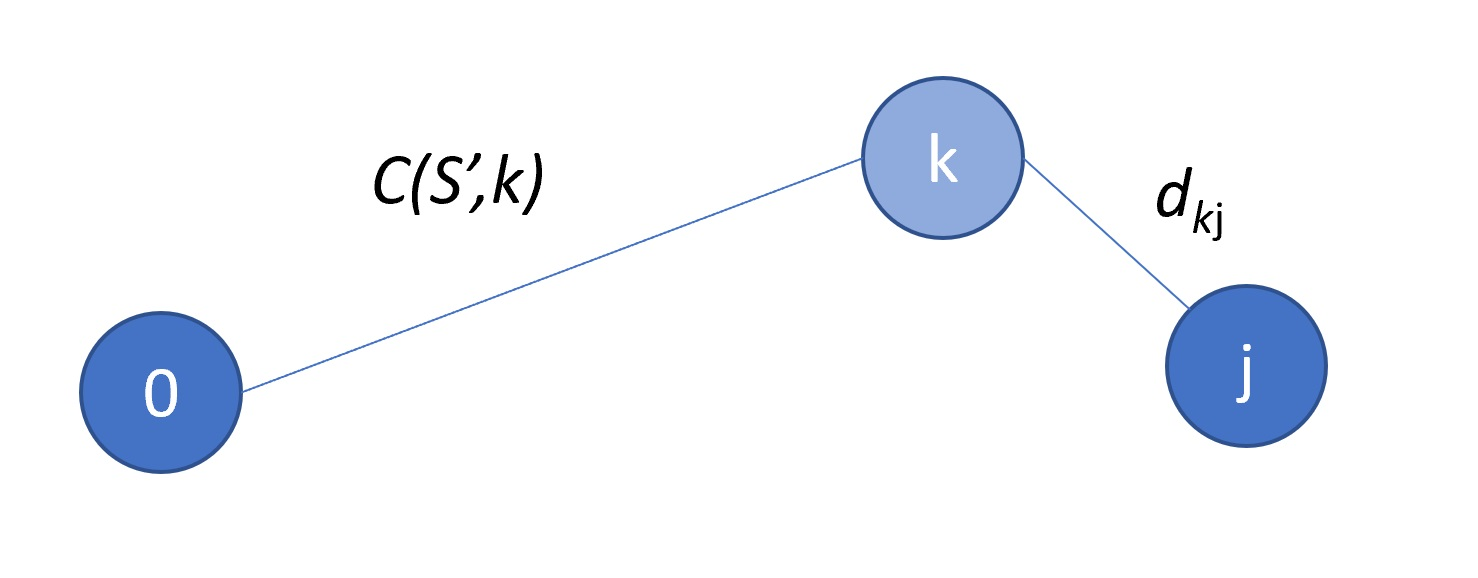
\includegraphics[height=3.5cm,valign=t]{dp_graphalgo.jpg}
\caption{Search of minimum cost for a subset of nodes \label{fig:dpgraphalgo}}
\end{figure}

\paragraph{Base case}\hfill \break
If $S'=\{0\}$, $$C(S',0)=0$$.

\paragraph{Implementation trick}\hfill \break
We use a bit field to code the subset of nodes selected in the set \{1,...n\}.
Each node j is code by the value $2^j$ when selected and 0 when not selected. 
\end{subsection}


\begin{subsection}{Pseudo code}
\begin{center}
	\colorbox[gray]{0.95}{
	\begin{minipage}{0.65\textwidth}
			\begin{algorithm}[H]
			\caption{Dynamic Programming Algorithm}
			\begin{algorithmic} 
			\STATE Initialization
			\FOR {j := 2 to n do}
			\STATE $C(\{j\},j)=0$
			\ENDFOR

			\FOR {$subsetsize$ := 2 to n-1}
			   \FOR {all $ S' \subseteq \{2,...,n \}$ with $|S'|=subsetsize$}
				  \FOR {all j in S'}
					 \STATE $C(S',j)=min_{k \in S'-\{j\}}\{C(S'-\{j\},k)+d_{kj}\}$
				  \ENDFOR
			   \ENDFOR
			\ENDFOR
			\STATE $mincost := min_{1<j \leq n}\{C(\{2,...,n\},j)+d_{j0}\}$
			\STATE return $mincost$
			\end{algorithmic}
			\end{algorithm}
	 \end{minipage}}
\end{center}

\end{subsection}




\begin{subsection}{Complexity}
   We need to build all the subsets of \{1,...,n\} i.e. $2^n$ subsets. For all nodes j of each subset (at most n nodes) and for all nodes k distinct from node j(at most n-1 nodes), we compute the cost of the sub paths terminated by node k for the subset deprived of node j.
Thus the time complexity is $2^n n^2$.
\newline{} In term of space complexity, if we use a bit field to code all subsets for each node $j \subseteq \{0,...,n\}$, the required space is $2^n (n+1)$.
\newline{} Nevertheless, we can note that to compute the cost for the subsets of size s, we only need the cost of the subsets of size (s-1). Thus the space complexity can be reduced to:
$$  max_{1<s<n}((s-1) \binom{n}{s-1} + s\binom{n}{s})$$
which is $O(2^n\sqrt n)$.\cite{wikidp}
\end{subsection}

\begin{subsection}{Performances}

The DP algorithm is run on a set of problems, symetric and asymetric, generated randomly with distance between 1 and 1000. 
The algorithm is first run with different graph sizes. Figure ~\ref{fig:dpgraphsize} shows that running time for both types of problem follow the theorical time complexity curve.
The performances are also measured with different sparsity levels. Figure ~\ref{fig:dpgraphsize} shows that the running time does not varies whith the sparsity. It is still necessary to examine all combinations of subsets.


\begin{figure}[H]
\centering
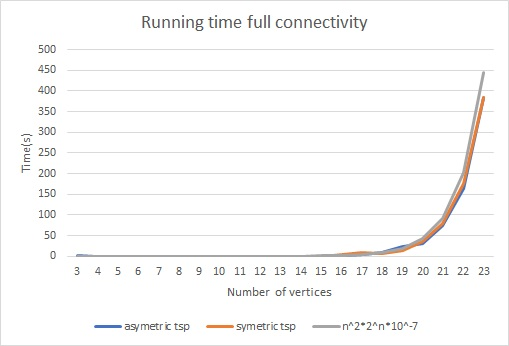
\includegraphics[height=5cm,valign=t]{dp_sizegraph.jpg}
\caption{Example of node selection \label{fig:dpgraphsize}}
\end{figure}

\begin{figure}[H]
\centering
\begin{subfigure}{.5\textwidth}
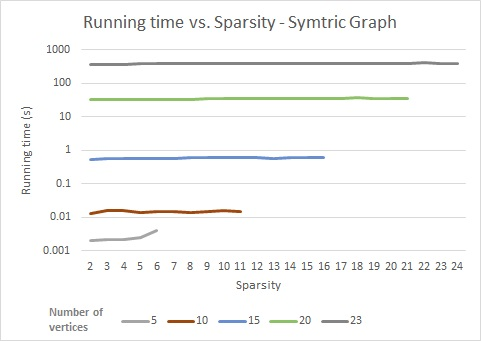
\includegraphics[height=5cm,valign=t]{dp_sym_sparsity.jpg}
\caption{Symetric problem \label{fig:dpgsparsitysym}}
\end{subfigure}%
\begin{subfigure}{.5\textwidth}
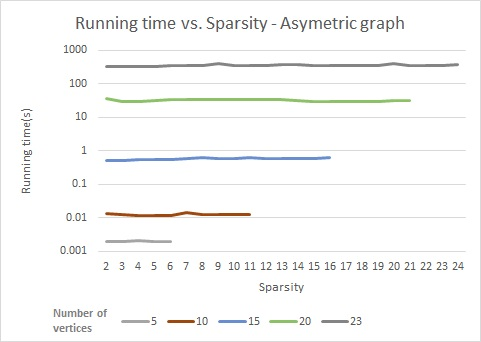
\includegraphics[height=5cm,valign=t]{dp_asym_sparsity.jpg}
\caption{Asymetric problem\label{fig:dpgsparsityasym}}
\end{subfigure}%
\caption{Sparsity impact study\label{fig:dpperf}}
\end{figure}

Memory usage is a limitation to running the dynamic programming algorithm. Only the smallest problems of TSLIB could be tested. The optimal solution is obtained each time as seen on Table \ref{table:dpt1}.

\begin{table}[H]
\centering
\footnotesize
\begin{tabular}{||c||c|c|c|l||}
\hline
\hline
\bf TSPLIB & \bf Run.time(s) & \bf Opt. Cost & \bf DP Cost & \bf Path \\
\hline
\hline
burma14 & 0.294 & 3323 & 3323 & [1, 2, 14, 3, 4, 5, 6, 12, 7, 13, 8, 11, 9, 10, 1]\\
gr17	& 3.285 & 2085 & 2085 &  [1, 4, 13, 7, 8, 6, 17, 14, 15, 3, 11, 10, 2, 5, 9, 12, 16, 1] \\
ulysses16 & 1.485	 & 6859 & 6859 & [1, 8, 4, 2, 3, 16, 10, 9, 11, 5, 15, 6, 7, 12, 13, 14, 1] \\
gr21& 86.711 & 2707 & 2707 &	[1, 7, 8, 6, 16, 5, 9, 3, 2, 21, 15, 14, 13, 18, 10, 17, 19, 20, \\
 & & & &   11, 4, 12, 1] \\
ulysses22 & 204.811 &	7013 & 7013 & [1, 8, 18, 4, 22, 17, 2, 3, 16, 21, 20, 19, 10, 9, 11, 5, 15, 6,\\
 & & & &    7, 12, 13, 14, 1]\\
gr24	& 849.022 & 1272 & 1272 &	[1, 12, 4, 23, 9, 13, 14, 20, 2, 15, 19, 18, 22, 17, 10, 5, 21, \\
 & & & &  8,24, 6, 7, 3, 11, 16, 1]   \\
\hline
\hline
\end{tabular}
\caption{TSLIB problem performances with dynamic programming}
\label{table:dpt1}
\end{table}

\end{subsection}

\end{document}


